\documentclass[11pt,letterpaper, onecolumn]{exam}
\usepackage{amsmath}
\usepackage{fancyvrb}
\usepackage{enumitem}
\usepackage{graphicx}
\usepackage{esvect}
\usepackage{bbm}
\usepackage{setspace}
\usepackage{arydshln}
\usepackage{tikz}
\usetikzlibrary{arrows.meta, positioning, calc}
\usepackage{cite}
\bibliographystyle{plain}
\usepackage{hyperref}
%\usepackage[utf8]{inputenc}
%\setlength{\parindent}{0pt}

\begin{document}

\title{\textbf{Mouse hippocampal dendritic spine dynamics over the estrous cycle as stochastic system}}
\author{EEMB 247/IQB 247 - Quant. Methods in Biology\\Dylan Martins}
\date{}

\maketitle

\section*{Abstract}
example text

\section{Introduction} % \cite{bib1}
\subsection{Neural plasticity and dendritic spine dynamics}
\subsection{The rodent estrous cycle}
\subsection{Modulation of spine dynamics by sex hormones}
% sex hormores and neural modulation
% dendritic spine modulation during estrus cycle
% hippocampus

\begin{figure}[h]
    \centering
    %\includegraphics[width=0.25\textwidth]{mesh}
    \caption{Neural plasticity, hippocampal dendritic spines, and the rodent estrous cycle. \textbf{a.} Neural plasticity....}
    \label{fig:intro}
\end{figure}

\section{Experimental methods}
Here, we use the publicly available dataset of \cite{nora}, which provides more detailed methodological details. A brief summary is provided here for context.
\subsection{Estrous cycle staging}
\subsection{Surgical procedures}
\subsection{Structural two-photon calcium imaging of dendritic spines}
\subsection{Spine classification}

\begin{figure}[h]
    \centering
    %\includegraphics[width=0.25\textwidth]{mesh}
    \caption{Overall title. \textbf{a.} estrousnet (adapted from \cite{estrousnet}), \textbf{b.} Schematic of hippocampal prisms implanted into mice. \textbf{c.} Strucural imaging of HP dendridic spines, segmentation, etc.. \textbf{d.} Spine classification schematic.}
    \label{fig:intro}
\end{figure}

\section{Modeling results}

\subsection{State variables and population flow}

\begin{figure}[h!]
\centering
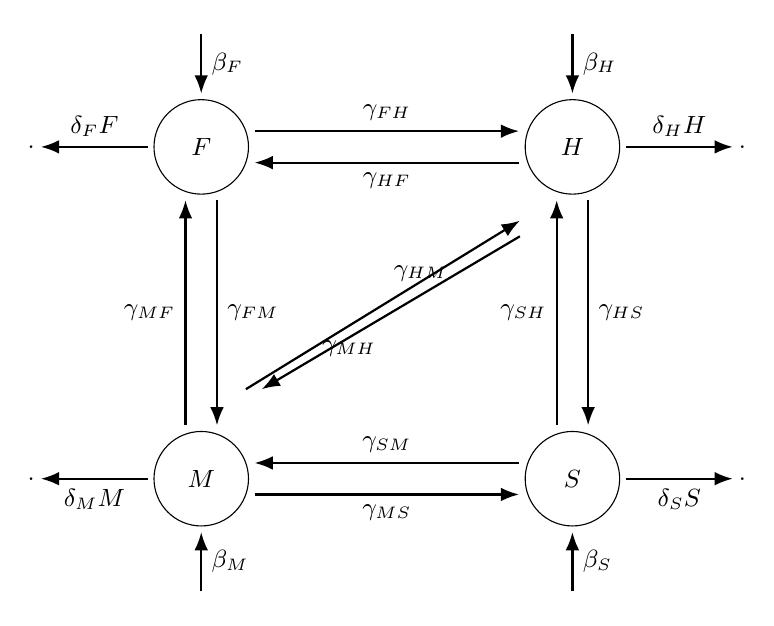
\begin{tikzpicture}[
  node distance=3cm and 3.5cm,
  state/.style={circle, draw, minimum size=1.2cm},
  arrow/.style={->, thick, >=Latex, shorten >=2pt, shorten <=2pt},
  font=\small
]

% Nodes
\node[state] (F) at (0, 0) {$F$};
\node[state] (H) [right=of F] {$H$};
\node[state] (S) [below=of H] {$S$};
\node[state] (M) [below=of F] {$M$};

% Dots for death events
\node[draw=none, minimum size=0pt, inner sep=0pt] (dotF) [left=1.5cm of F] {.};
\node[draw=none, minimum size=0pt, inner sep=0pt] (dotH) [right=1.5cm of H] {.};
\node[draw=none, minimum size=0pt, inner sep=0pt] (dotS) [right=1.5cm of S] {.};
\node[draw=none, minimum size=0pt, inner sep=0pt] (dotM) [left=1.5cm of M] {.};

% Births (up/down arrows from nowhere)
\draw[arrow] ($(F)+(0,1.5)$) -- (F) node[midway, right] {$\beta_F$};
\draw[arrow] ($(H)+(0,1.5)$) -- (H) node[midway, right] {$\beta_H$};
\draw[arrow] ($(S)+(0,-1.5)$) -- (S) node[midway, right] {$\beta_S$};
\draw[arrow] ($(M)+(0,-1.5)$) -- (M) node[midway, right] {$\beta_M$};

% Deaths
\draw[arrow] (F.west) -- (dotF) node[midway, above] {$\delta_F F$};
\draw[arrow] (H.east) -- (dotH) node[midway, above] {$\delta_H H$};
\draw[arrow] (S.east) -- (dotS) node[midway, below] {$\delta_S S$};
\draw[arrow] (M.west) -- (dotM) node[midway, below] {$\delta_M M$};

% Transitions (offset bidirectional)

% F <-> H
\draw[arrow] ($(F.east)+(0,0.2)$) -- ($(H.west)+(0,0.2)$) node[midway, above] {$\gamma_{FH}$};
\draw[arrow] ($(H.west)-(0,0.2)$) -- ($(F.east)-(0,0.2)$) node[midway, below] {$\gamma_{HF}$};

% F <-> S
%\draw[arrow] ($(F.east)+(0,0.2)$) -- ($(S.west)+(0,0.2)$) node[midway, above] {$\gamma_{FS}$};
%\draw[arrow] ($(S.west)-(0,0.2)$) -- ($(F.east)-(0,0.2)$) node[midway, below] {$\gamma_{SF}$};

% F <-> M
\draw[arrow] ($(F.south)+(0.2,0)$) -- ($(M.north)+(0.2,0)$) node[midway, right] {$\gamma_{FM}$};
\draw[arrow] ($(M.north)-(0.2,0)$) -- ($(F.south)-(0.2,0)$) node[midway, left] {$\gamma_{MF}$};

% H <-> S
\draw[arrow] ($(H.south)+(0.2,0)$) -- ($(S.north)+(0.2,0)$) node[midway, right] {$\gamma_{HS}$};
\draw[arrow] ($(S.north)-(0.2,0)$) -- ($(H.south)-(0.2,0)$) node[midway, left] {$\gamma_{SH}$};

% H <-> M
\draw[arrow] ($(H.west)+(0,-1.1)$) -- ($(M.east)+(0.1,1.1)$) node[pos=0.25, left] {$\gamma_{HM}$};
\draw[arrow] ($(M.east)+(-0.1,1.1)$) -- ($(H.west)+(0,-0.9)$) node[pos=0.25, right] {$\gamma_{MH}$};

% S <-> M
\draw[arrow] ($(S.west)+(0,0.2)$) -- ($(M.east)+(0,0.2)$) node[midway, above] {$\gamma_{SM}$};
\draw[arrow] ($(M.east)-(0,0.2)$) -- ($(S.west)-(0,0.2)$) node[midway, below] {$\gamma_{MS}$};

\end{tikzpicture}
\caption{Arrows stop at circle edges; opposing transitions are offset for clarity.}
\end{figure}

\subsection{Estradiol concentration over the estrus cycle}\label{subsec2}
The four-harmonic Fourier series for estradiol concentration over the estrus cycle can be expressed as
\begin{equation}
f(t)=a_0+\sum_{n=1}^{4}a_n sin\frac{2\pi n t}{p}+b_n cos\frac{2\pi nt}{p}
\label{eq:estradiol_fourier}
\end{equation}
where the values of parameters are $a_0=65.07, a_1=-35.94, b_1=68.53, a_2=-71.13, b_2=-2.5, a_3=-43.44, b_3-66.03,  a_4=11.67, b_4=-55.08$.

Here, $f(t)$ predicts the endogenous concentration of E2 estradiol in units of $pg/mL$ as a function of time, with time in units of days aligned to diestrus ($0\leq t < 1$), proestrus ($1\leq t < 2$), estrus ($2\leq t < 3$), and metestrus ($3\leq t < 4$) stages. In these timesteps, ovulation occurs at $t=2.25$ and given a period of $p=4$ in equation \eqref{eq:estradiol_fourier}, $t=0$ and $t=4$ are of equivalent value.

\begin{figure}[h]
    \centering
    %\includegraphics[width=0.25\textwidth]{mesh}
    \caption{Overall title. \textbf{a.} }
    \label{fig:intro}
\end{figure}

\subsection{Spine class transition probabilities}

Let $\beta_x$ be the spontaneous growth rate new spines, for $x \in \{F, H, S, M\}$, $\delta_x$ the per-individual death rate, and $\gamma_{x \to y}$ the per-individual transition rate from state $x$ to $y$, for all distinct $x, y \in \{F, H, S, M\}$. The growth rates $\beta_x$ are treated as independent from the current population size.

Each entry in the transition matrix $Q\in \mathbbm{R}^{5x5}$ gives the frequency of transition from the current state $x$ to the next state $y$ as $Q_{x\to y}$. The set of possible states is defined as $\mathcal{S}=\{NS,F,H,S,M\}$ where $NS$ indicates no spine to allow for growth and pruning terms. Rows of $Q$ are the current state and columns of $Q$ are the target state. The zeroth row represents outgoing transitions from the $NS$ state, i.e., new growth, while the zeroth column represents incoming transitions to the $NS$ state, i.e., existing spines being pruned away. The diagonal entries, $\lambda_x$ represent the total rate of leaving state $x$, where
\[\lambda_x=\delta_x+\sum_{y\neq x}\gamma_{x\to y}\]
The complete transition matrix takes the form of
\[Q = \begin{bmatrix}
\delta_M & \gamma_{M \to F} & \gamma_{M \to H} & \gamma_{M \to S} & -\lambda_M \\
\delta_S & \gamma_{S \to F} & \gamma_{S \to H} & -\lambda_S & \gamma_{S \to M} \\
\delta_H & \gamma_{H \to F} & -\lambda_H & \gamma_{H \to S} & \gamma_{H \to M} \\
\delta_F & -\lambda_F & \gamma_{F \to H} & \gamma_{F \to S} & \gamma_{F \to M} \\
0 & \beta_F & \beta_H & \beta_S & \beta_M
\end{bmatrix}\]
However, $Q$ must be calculated for all four of the estrous cycle stage transitions, i.e., $Q_x$ for $x\in\{D,P,E,M\}$ Following the approach in equations ??? and ???, the following transition probabilities were computed:

\begin{figure}[h]
    \centering
    %\includegraphics[width=0.25\textwidth]{mesh}
    \caption{Overall title. \textbf{a.} }
    \label{fig:intro}
\end{figure}

\subsection{Spine dynamics as a continuous-time system}

The expression for the four continuous-time state equations is
\begin{equation}
\begin{split}
\frac{dF}{dt}= &\beta_F - \delta_FF+\gamma_{HF}H+\gamma_{SF}S+\gamma_{MF}M-F(\gamma_{FH}+\gamma_{FS}+\gamma_{FM})\\
\frac{dH}{dt} = &\beta_H - \delta_H H + \gamma_{FH} F + \gamma_{SH} S + \gamma_{MH} M - H (\gamma_{HF} + \gamma_{HS} + \gamma_{HM})\\
\frac{dS}{dt} = &\beta_S - \delta_S S + \gamma_{FS} F + \gamma_{HS} H + \gamma_{MS} M - S (\gamma_{SF} + \gamma_{SH} + \gamma_{SM})\\
\frac{dM}{dt} = &\beta_M - \delta_M M + \gamma_{FM} F + \gamma_{HM} H + \gamma_{SM} S - M (\gamma_{MF} + \gamma_{MH} + \gamma_{MS})
\end{split}
\end{equation}

However, this can be expressed as a stochastic system of discrete events, where $F,H,S,M\in \mathbbm{Z}_{\geq0}$. The system described by these equations involve 20 possible events affecting the state vector
\[X(t)=\begin{bmatrix}F(t)\\H(t)\\S(t)\\M(t)\end{bmatrix}\]

\begin{table}[h!]
\centering \resizebox{\textwidth}{!}{
\begin{tabular}{|c|c|c|c||c|c|c|c|}
\hline
\textbf{\#} & \textbf{Event} & \textbf{Definition} & \textbf{Vector}&\textbf{\#} & \textbf{Event} & \textbf{Definition} & \textbf{Vector}\\
\hline
\hline
1 & New $F$ grown & $k_1=\beta_F$ & $v_1=\begin{bmatrix}1\\0\\0\\0\end{bmatrix}$ & 11 & $M$ transitions to $F$ & $k_{11}=\gamma_{MF}M$ & $v_{11}=\begin{bmatrix}1\\0\\0\\-1\end{bmatrix}$\\
\hline
2 & New $H$ grown & $k_2=\beta_H$ & $v_2=\begin{bmatrix}0\\1\\0\\0\end{bmatrix}$ & 12 & $F$ transitions to $H$ & $k_{12}=\gamma_{FH}F$ & $v_{12}=\begin{bmatrix}-1\\1\\0\\0\end{bmatrix}$\\
\hline
3 & New $S$ grown & $k_3=\beta_S$ & $v_3=\begin{bmatrix}0\\0\\1\\0\end{bmatrix}$ & 13 & $F$ transitions to $S$ & $k_{13}=\gamma_{FS}F$ & $v_{13}=\begin{bmatrix}-1\\0\\1\\0\end{bmatrix}$\\
\hline
4 & New $M$ grown & $k_4=\beta_M$ & $v_4=\begin{bmatrix}0\\0\\0\\1\end{bmatrix}$ & 14 & $F$ transitions to $M$ & $k_{14}=\gamma_{FM}F$ & $v_{14}=\begin{bmatrix}-1\\0\\0\\1\end{bmatrix}$\\
\hline
5 & Existing $F$ pruned & $k_5=\delta_FF$ & $v_5=\begin{bmatrix}-1\\0\\0\\0\end{bmatrix}$ & 15 & $S$ transitions to $H$ & $k_{15}=\gamma_{SH}S$ & $v_{15}=\begin{bmatrix}0\\1\\-1\\0\end{bmatrix}$\\
\hline
6 & Existing $H$ pruned & $k_6=\delta_HH$ & $v_6=\begin{bmatrix}0\\-1\\0\\0\end{bmatrix}$ & 16 & $M$ transitions to $H$ & $k_{16}=\gamma_{MH}M$ & $v_{16}=\begin{bmatrix}0\\1\\0\\-1\end{bmatrix}$\\
\hline
7 & Existing $S$ pruned & $k_7=\delta_SS$ & $v_7=\begin{bmatrix}0\\0\\-1\\0\end{bmatrix}$ & 17 & $H$ transitions to $S$ & $k_{17}=\gamma_{HS}H$ & $v_{17}=\begin{bmatrix}0\\-1\\1\\0\end{bmatrix}$\\
\hline
8 & Existing $M$ pruned & $k_8=\delta_MM$ & $v_8=\begin{bmatrix}0\\0\\0\\-1\end{bmatrix}$ & 18 & $M$ transitions to $S$ & $k_{18}=\gamma_{MS}M$ & $v_{18}=\begin{bmatrix}0\\0\\1\\-1\end{bmatrix}$\\
\hline
9 & $H$ transitions to $F$ & $k_9=\gamma_{HF}H$ & $v_9=\begin{bmatrix}1\\-1\\0\\0\end{bmatrix}$ & 19 & $H$ transitions to $M$ & $k_{19}=\gamma_{HM}H$ & $v_{19}=\begin{bmatrix}0\\-1\\0\\1\end{bmatrix}$\\
\hline
10 & $S$ transitions to $F$ & $k_{10}=\gamma_{SF}S$ & $v_{10}=\begin{bmatrix}1\\0\\-1\\0\end{bmatrix}$ & 20 & $S$ transitions to $M$ & $k_{20}=\gamma_{SM}S$ & $v_20=\begin{bmatrix}0\\0\\-1\\1\end{bmatrix}$\\
\hline
\end{tabular}}
\end{table}

Using these event definitions, we can reformulate the state equations as a stochastic birth-death-transition process where the probability of having $n$ spines of type $F$ at time $t$ is given by $p_n^{F}(t)$.

\begin{equation}
\begin{split}
\frac{dp_n^F}{dt} &= k_1p_{n-1}^F + k_9p_{n-1}^F + k_{10}p_{n-1}^F + k_{11}p_{n-1}^F - (k_5 + k_{12} + k_{13} + k_{14})p_n^F \\
\frac{dp_n^H}{dt} &= k_2p_{n-1}^H + k_{12}p_{n-1}^H + k_{15}p_{n-1}^H + k_{16}p_{n-1}^H- (k_6 + k_9 + k_{17} + k_{19})p_n^H \\
\frac{dp_n^S}{dt} &= k_3p_{n-1}^S + k_{13}p_{n-1}^S + k_{17}p_{n-1}^S + k_{18}p_{n-1}^S - (k_7 + k_{10} + k_{15} + k_{20})p_n^S \\
\frac{dp_n^M}{dt} &= k_4p_{n-1}^M+ k_{14}p_{n-1}^M + k_{19}p_{n-1}^M+ k_{20}p_{n-1}^M- (k_8 + k_{11} + k_{16} + k_{18})p_n^M\\
\end{split}
\end{equation}

This is modeled using the Gillespie stochastic simulation algorithm. However, in order to model spine fluctuations through time as endogenous estradiol concentrations fluctuate over time, the simulation must include a function for the effect of this non-homogenous ``environmental'' function, following Equation \eqref{eq:estradiol_fourier}.



%\begin{equation}
%\begin{split}
%\label{eq:master}
%\frac{dP_{f,h,s,m}}{dt}&= \beta_F P_{f-1,h,s,m} + \beta_H P_{f,h-1,s,m} + \beta_S P_{f,h,s-1,m} + \beta_M P_{f,h,s,m-1}\\
%&+ (f+1)\delta_F P_{f+1,h,s,m} + (h+1)\delta_H P_{f,h+1,s,m}+ (s+1)\delta_S P_{f,h,s+1,m}\\
%& \hspace{50pt}+ (m+1)\delta_M P_{f,h,s,m+1}\\
%&+ (f+1)\gamma_{F \to H} P_{f+1,h-1,s,m} + (f+1)\gamma_{F \to S} P_{f+1,h,s-1,m}\\
%&\hspace{50pt}+(f+1)\gamma_{F \to M} P_{f+1,h,s,m-1}\\
%&+ (h+1)\gamma_{H \to F} P_{f-1,h+1,s,m} + (h+1)\gamma_{H \to S} P_{f,h+1,s-1,m}\\
%&\hspace{50pt}+ (h+1)\gamma_{H \to M} P_{f,h+1,s,m-1}\\
%&+ (s+1)\gamma_{S \to F} P_{f-1,h,s+1,m} + (s+1)\gamma_{S \to H} P_{f,h-1,s+1,m}\\
%&\hspace{50pt}+ (s+1)\gamma_{S \to M} P_{f,h,s+1,m-1}\\
%&+ (m+1)\gamma_{M \to F} P_{f-1,h,s,m+1} + (m+1)\gamma_{M \to H} P_{f,h-1,s,m+1}\\
%&\hspace{50pt}+ (m+1)\gamma_{M \to S} P_{f,h,s-1,m+1} \\
%&- \Big[ \beta_F + \beta_H + \beta_S + \beta_M\\
%&\hspace{50pt}+f(\delta_F + \gamma_{F \to H} + \gamma_{F \to S} + \gamma_{F \to M}) \\
%&\hspace{50pt} + h(\delta_H + \gamma_{H \to F} + \gamma_{H \to S} + \gamma_{H \to M}) \\
%&\hspace{50pt} + s(\delta_S + \gamma_{S \to F} + \gamma_{S \to H} + \gamma_{S \to M}) \\
%&\hspace{50pt} + m(\delta_M + \gamma_{M \to F} + \gamma_{M \to H} + \gamma_{M \to S})\\
%&\hspace{100pt}\Big] P_{f,h,s,m}
%\end{split}
%\end{equation}


\section*{References}
\begin{itemize}[label={}]
\item Legault, G. \& Melbourne, B.A. Accounting for environmental change in continuous-time stochastic population models. \textit{Theor Ecol} 12, 31--48 (2019). \url{https://doi.org/10.1007/s12080-018-0386-z}
\item Wolcott, N.S., Sit, K.K., Raimondi, G. \textit{et al.} Automated classification of estrous stage in rodents using deep learning. \textit{Sci Rep} 12, 17685 (2022). \url{https://doi.org/10.1038/s41598-022-22392-w}
\item Wolcott, N.S., Redman, W.T., Karpinska M. \textit{et al.} The estrous cycle modulates hippocampal spine dynamics, dendritic processing, and spatial coding. \textit{Neuron} 113, 1-13 (2025). \url{https://doi.org/10.1016/j.neuron.2025.04.014}
\item Woolley, C.S., Gould, E., Grankfurt, M., \& McEwen, B.S. Naturally occurring fluctuation in dendritic spine density on adult hippocampal pyramidal neurons. \textit{J. Neurosci.} 10(12) 4035--4039 (1990). \url{https://doi.org/10.1523/JNEUROSCI.10-12-04035.1990}
\item Donner, N.C., Lowry, C.A. Sex differences in anxiety and emotional behavior. \textit{Pflugers Arch - Eur J Physiol} 465, 601–626 (2013). \url{https://doi.org/10.1007/s00424-013-1271-7}
\end{itemize}
% https://www.sciencedirect.com/science/article/pii/S001664801100428X?via%3Dihub
% https://pmc.ncbi.nlm.nih.gov/articles/PMC3471296/#ref-list1
% https://pmc.ncbi.nlm.nih.gov/articles/PMC2921935/#:~:text=%5BE2%5D%20in%20male%20mice%20is,OVX%20sham%2C%20and%20males).&text=%5BE2%5D%20measurements%20were%20performed%20in,sham%20(P%3C0.05).
% https://www.sciencedirect.com/science/article/pii/S001664801100428X?via%3Dihub
% https://pmc.ncbi.nlm.nih.gov/articles/PMC3471296/#ref-list1







\end{document}